% Unofficial UofT Poster template.
% A fork of the UMich template https://www.overleaf.com/latex/templates/university-of-michigan-umich-poster-template/xpnqzzxwbjzc
% which is fork of the MSU template https://www.overleaf.com/latex/templates/an-unofficial-poster-template-for-michigan-state-university/wnymbgpxnnwd
% which is a fork of https://www.overleaf.com/latex/templates/an-unofficial-poster-template-for-new-york-university/krgqtqmzdqhg
% which is a fork of https://github.com/anishathalye/gemini
% also refer to https://github.com/k4rtik/uchicago-poster

\documentclass[final]{beamer}

% ====================
% Packages
% ====================

\usepackage[T1]{fontenc}
% lualatex is Unicode-native; no inputenc needed
\usepackage{lmodern}
% Narrow two-panel layout: portrait, ~A0 width
\usepackage[size=custom, width=91,height=122, scale=1.2]{beamerposter}
\usetheme{gemini}
\usecolortheme{uoft}
\usepackage{graphicx}
\usepackage{booktabs}
\usepackage{tikz}
\usetikzlibrary{arrows.meta,calc,positioning,decorations.pathmorphing,decorations.markings,3d,backgrounds,shapes.geometric,fit}
\usepackage{pgfplots}
\pgfplotsset{compat=1.14}
\usepackage{anyfontsize}
\usepackage[nolinks]{qrcode}

% ====================
% Animation companion page (GitHub Pages)
% ====================
% Update this URL to the published GitHub Pages URL of /docs.
\newcommand{\animationurl}{https://YOUR-GITHUB-USERNAME.github.io/YOUR-REPOSITORY-NAME/}
\newsavebox{\animationqrbox}
\AtBeginDocument{%
  \sbox{\animationqrbox}{\qrcode[height=4cm,level=H]{\animationurl}}%
}

% ====================
% Lengths
% ====================

% If you have N columns, choose \sepwidth and \colwidth such that
% (N+1)*\sepwidth + N*\colwidth = \paperwidth
% Two-column layout: 3*sep + 2*col = paperwidth, with sep = 0.03
\newlength{\sepwidth}
\newlength{\colwidth}
\setlength{\sepwidth}{0.03\paperwidth}
\setlength{\colwidth}{0.455\paperwidth}

\newcommand{\separatorcolumn}{\begin{column}{\sepwidth}\end{column}}

% ====================
% Title
% ====================

\title{Quantum Fisher information as a probe of multipartite entanglement
in frustrated quantum magnets}

\author{Zhengbang Zhou, Chengkang Zhou, Menghan Song, Zi Yang Meng, and Yong Baek Kim}

\institute[shortinst]{Department of Physics, University of Toronto
\quad\textbullet\quad CIFAR Quantum Materials Program}

% ====================
% Footer (optional)
% ====================

\footercontent{
  \href{https://arxiv.org/abs/2510.14813}{arXiv:2510.14813} \hfill
  CIFAR Quantum Materials Program Meeting 2026 \hfill
  \href{mailto:zhengbang.zhou@mail.utoronto.ca}{zhengbang.zhou@mail.utoronto.ca}}
% (can be left out to remove footer)

% ====================
% Logo (optional)
% ====================

% use this to include logos on the left and/or right side of the header:
% Left: institution logo
\logoleft{
\includegraphics[height=8cm]{logos/logo.png}}
% Right: QR codes for the two papers
\logoright{%
  \begin{tabular}{cc}
    \qrcode[height=6cm,level=H]{https://arxiv.org/abs/2510.14813} &
    \qrcode[height=6cm,level=H]{https://arxiv.org/abs/2603.19951}\\[0.3ex]
    {\scriptsize\color{white}arXiv:2510.14813} &
    {\scriptsize\color{white}arXiv:2603.19951}\\
  \end{tabular}}
% ====================
% Body
% ====================

\begin{document}



\begin{frame}[t]
\begin{columns}[t]
\separatorcolumn

\begin{column}{\colwidth}

  \begin{block}{Motivation}

Multipartite entanglement is a defining hallmark of strongly correlated
    quantum phases of matter, but it is difficult to access
    experimentally. The \textbf{quantum Fisher information} (QFI) density
    \[
      f_{Q,\alpha}(\mathbf{q}) = \frac{4}{\pi}\!\int_0^{\infty}\!\!d\omega\,
        \tanh\!\left(\frac{\omega}{2T}\right)\,\chi''_{\alpha}(\mathbf{q},\omega),
    \]
    can be extracted from inelastic scattering. Here
    $\chi''_{\alpha}(\mathbf{q},\omega)=\mathrm{Im}\,
    \langle O^{\alpha}_{\mathbf{q}};O^{\alpha\dagger}_{\mathbf{q}}\rangle_{\omega}$
    is the dissipative susceptibility of any spin component
    $\alpha\in\{x,y,z\}$ at any momentum $\mathbf{q}$, with
    $O^{\alpha}_{\mathbf{q}}=N^{-1/2}\sum_i
    e^{-i\mathbf{q}\cdot\mathbf{r}_i}S_i^\alpha$.
    A value $f_Q > k$ certifies at least $k{+}1$-partite entanglement.

    \begin{center}
    \resizebox{0.76\linewidth}{!}{%
    \begin{tikzpicture}[x=1cm,y=1cm,
        spin/.style={circle,draw=UofTBlue,fill=white,
             inner sep=0pt,minimum size=0.78cm,line width=1pt},
        block/.style={draw=UofTLightBlue,line width=1.1pt,
                      rounded corners=7pt,inner sep=4.6pt},
        witness/.style={draw=UofTBlue,line width=1.6pt,
                        rounded corners=8pt,
                        fill=UofTLightAccent,fill opacity=0.6,
                        inner sep=5.6pt},
      lbl/.style={font=\footnotesize\bfseries,text=UofTBlue},
      note/.style={font=\footnotesize,text=UofTBlue,align=left}]
      \node[lbl,anchor=west] at (0,7.45)
        {$1$-, $2$-, and $3$-producible partitions};

      \foreach \i in {0,...,7}{
        \node[spin] (a\i) at (\i*1.15,5.9) {};
        \node[block,fit=(a\i)] {};
      }
      \node[lbl,anchor=east] at (-0.4,5.9) {$1$-body};

      \foreach \i in {0,...,7}{
        \node[spin] (b\i) at (\i*1.15,4.1) {};
      }
      \foreach \j/\k in {0/1,2/3,4/5,6/7}{
        \node[block,fit=(b\j)(b\k)] {};
      }
      \node[lbl,anchor=east] at (-0.4,4.1) {$2$-body};

      \foreach \i in {0,...,7}{
        \node[spin] (c\i) at (\i*1.15,2.3) {};
      }
      \node[block,fit=(c0)(c1)(c2)] {};
      \node[block,fit=(c3)(c4)(c5)] {};
      \node[block,fit=(c6)(c7)] {};
      \node[lbl,anchor=east] at (-0.4,2.3) {$3$-body};

      \draw[-{Latex[length=5mm]},line width=1.5pt,UofTBlue]
        (9.55,4.1) -- (11.3,4.1);
      \node[lbl] at (10.45,4.85) {$f_Q>k$};

      \foreach \i in {0,...,7}{
        \node[spin] (d\i) at (12.45+\i*1.15,4.1) {};
      }
      \node[witness,fit=(d2)(d3)(d4)(d5)] {};
      \node[lbl] at (16.5,6.0) {certifies a $(k{+}1)$-body block};
      \node[note,anchor=west] at (12.0,2.15)
        {QFI lower-bounds the minimum block size that must be present.};
    \end{tikzpicture}}
    \end{center}

    \begin{itemize}
      \item \textbf{Goal.} Use QFI as a sharp, falsifiable diagnostic of
        spin-liquid candidates and unconventional critical points.
      \item \textbf{Methodologies.} Stochastic series expansion QMC + stabilized
        analytical continuation (SAC), exact diagonalisation, and finite-size
        scaling.
    \end{itemize}

  \end{block}

 \begin{block}{Quantum Spin Ice}

   We consider the simplified XXZ model which hosts the dipolar Quantum Spin Ice (QSI)
   in the local frame:
\begin{equation}
\label{eq:XXZ_Ham}
H = J_{\mathrm{z}}\sum_{\langle i, j\rangle} S_i^{\mathrm{z}} S_j^{\mathrm{z}}
- J_{\pm}\sum_{\langle i, j\rangle}\left(S_i^{+} S_j^{-}+S_i^{-} S_j^{+}\right)
\end{equation}

 \end{block}

 \begin{figure}
     \centering
     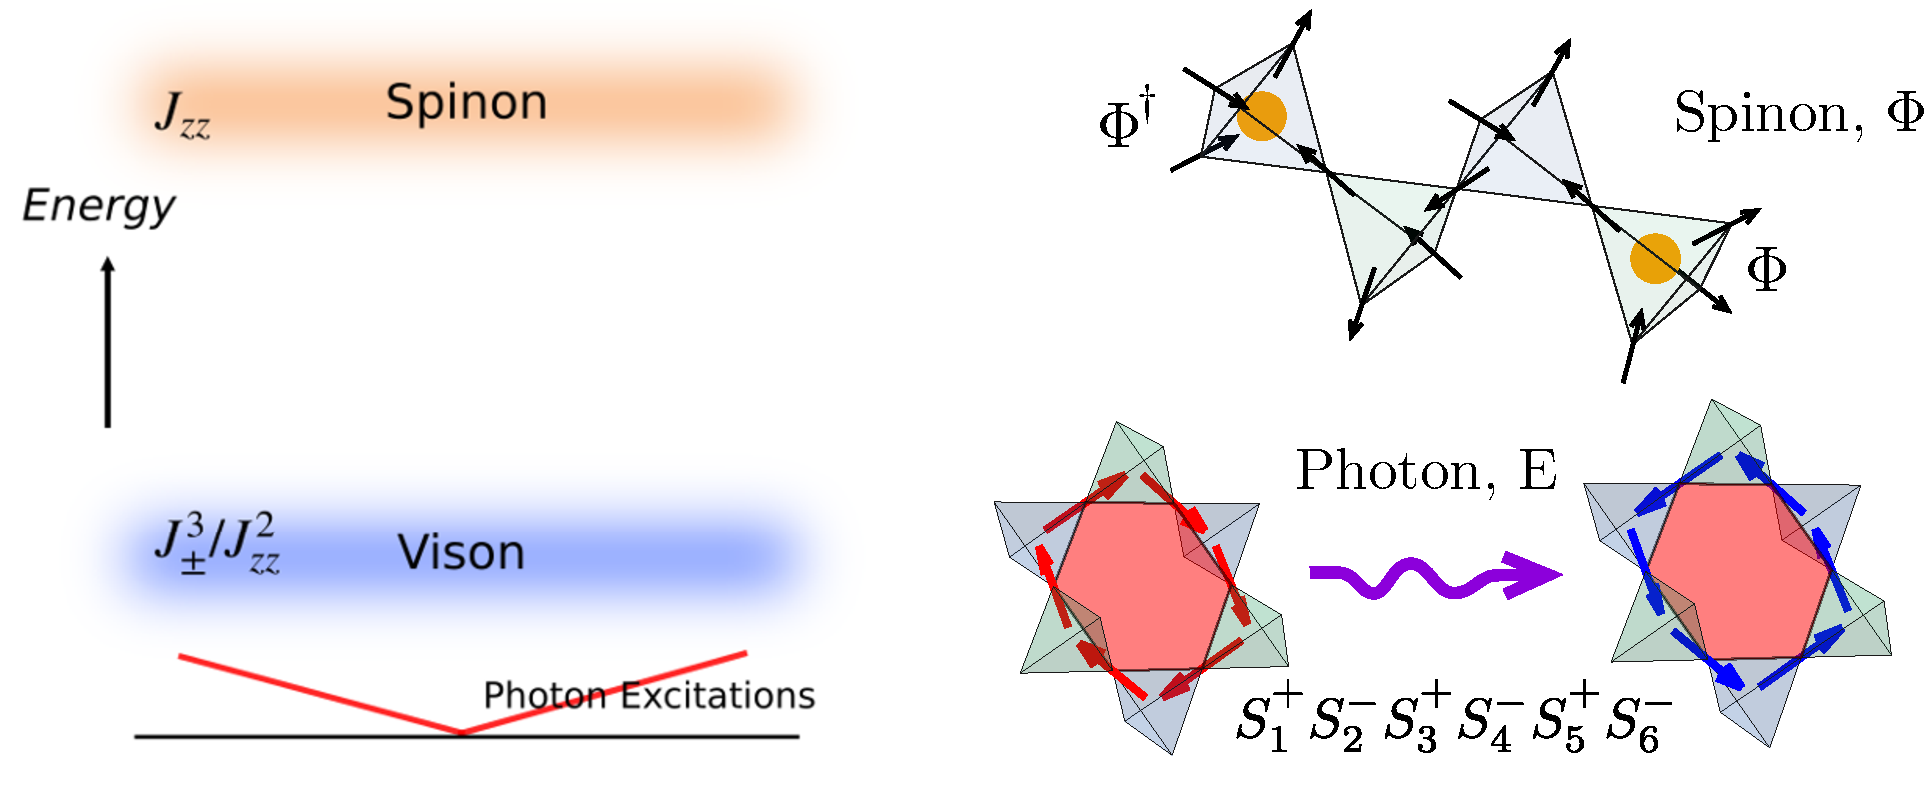
\includegraphics[width=0.75\linewidth]{figures/Fig1.pdf}
     \caption{Excitation hierarchy of QSI}
     \label{fig:placeholder}
 \end{figure}


  \begin{block}{$f_Q$: more than a restructured integral}

    The Lehmann representation shows what the QFI keeps and what it discards:

    \begin{minipage}[c]{0.72\linewidth}
    \[
      f_{Q,\alpha}(\mathbf{q})
      = \frac{2}{Z}\sum_{m,n}
        \frac{\bigl(e^{-\beta E_n}-e^{-\beta E_m}\bigr)^2}
             {e^{-\beta E_n}+e^{-\beta E_m}}
        \bigl|\langle m|O^{\alpha}_{\mathbf{q}}|n\rangle\bigr|^2.
    \]
    \end{minipage}\hfill
    \begin{minipage}[c]{0.24\linewidth}
      \centering
      \usebox{\animationqrbox}\par
      {\scriptsize Scan for $S^xS^x$ and $S^zS^z$ animations.}
    \end{minipage}

    \begin{itemize}
      \item \textbf{No classical static piece.} Diagonal $m=n$ terms vanish, so
        ordinary thermal variance at $\omega=0$ is not certified as entanglement.
      \item \textbf{Low-frequency thermal noise is filtered.}
        $\tanh(\omega/2T)\sim\omega/2T$ suppresses slow classical fluctuations.
    \end{itemize}

    \begin{figure}
        \centering
        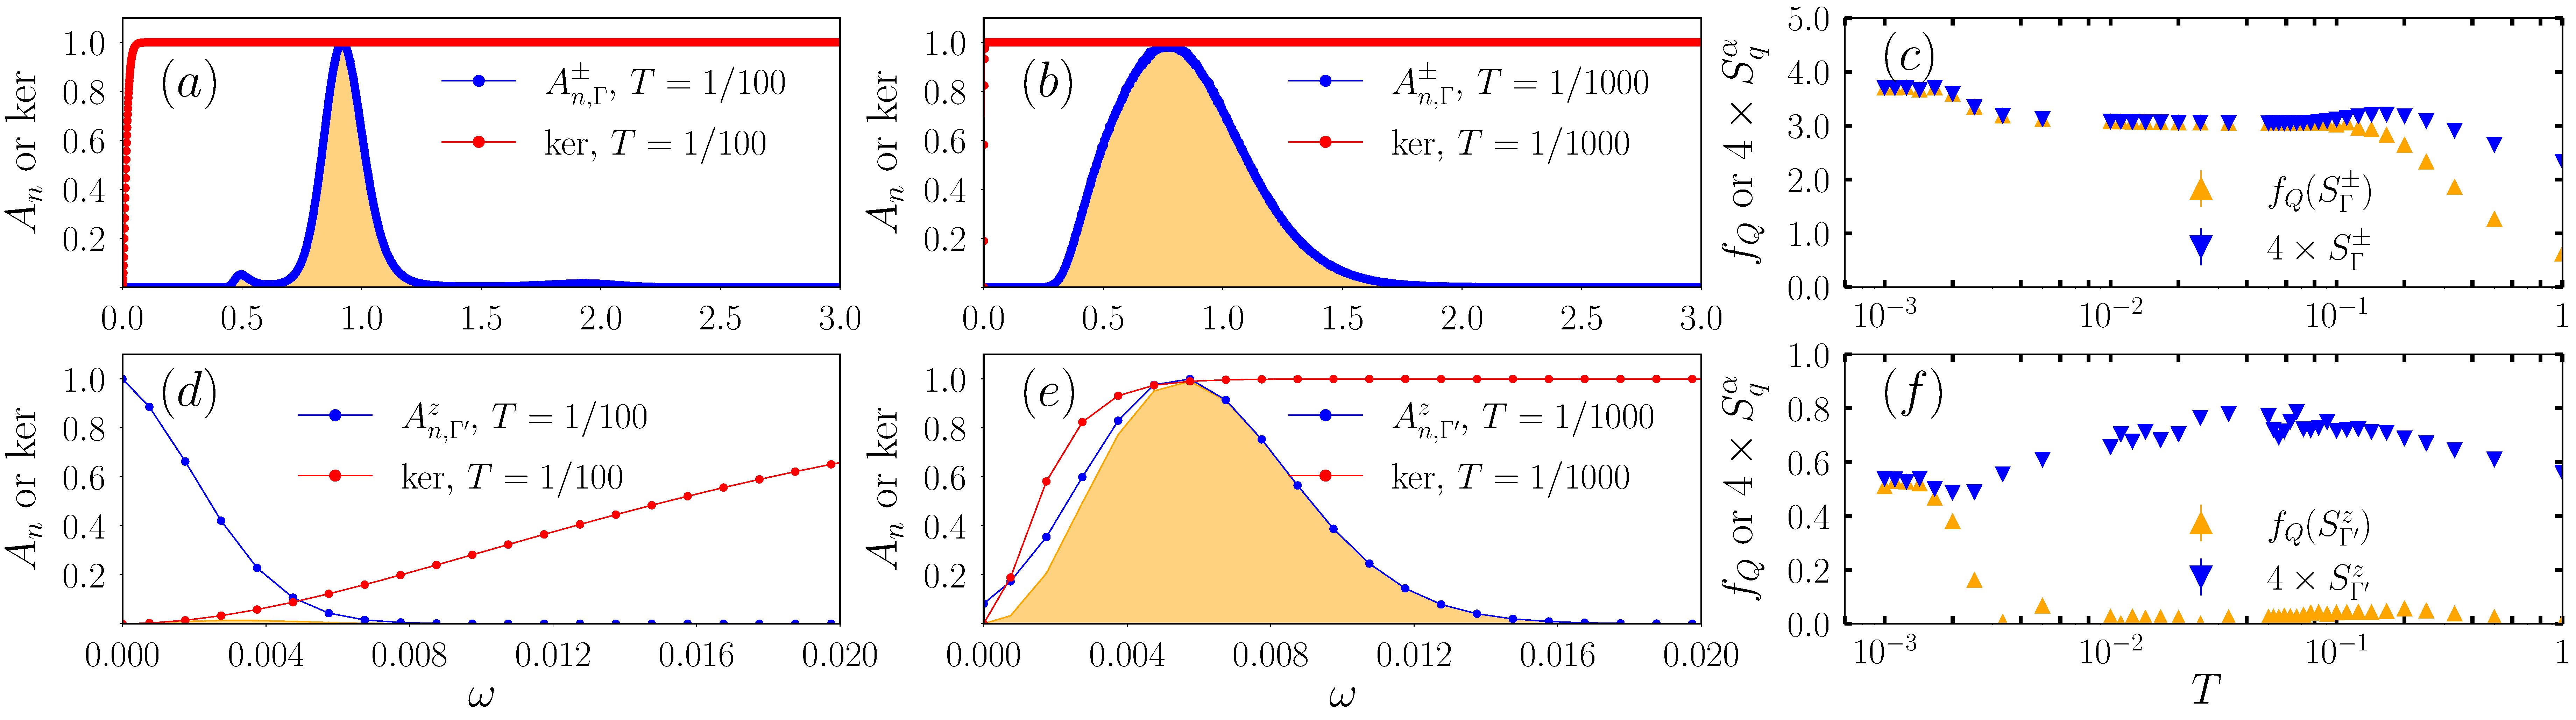
\includegraphics[width=\linewidth]{figures/Fig_re01.pdf}
        \caption{The comparison between QFI and static structure factor. $A^\alpha_n$ shows the dynamical structure factor and $\text{ker}=\tanh(\omega/2T)$ filters show slow classical fluctuation depending on the temperature.}
        \label{fig:placeholder}
    \end{figure}

  \end{block}
  \begin{block}{References \& acknowledgements}

    \footnotesize
    [1] P.\ Hauke, M.\ Heyl, L.\ Tagliacozzo, P.\ Zoller, Nat.\ Phys.\ 12,
    778 (2016).\par
    [2] M.\ J.\ P.\ Gingras, P.\ A.\ McClarty, Rep.\ Prog.\ Phys.\ 77,
    056501 (2014).\par
    [3] P.\ Hyllus \emph{et al.}, Phys.\ Rev.\ A 85, 022321 (2012).\par
    [4] G.\ T\'oth, Phys.\ Rev.\ A 85, 022322 (2012).
  \end{block}
\end{column}

\separatorcolumn

\begin{column}{\colwidth}

  \begin{block}{Quantum Fisher Information Heatmap}

  \begin{figure}
      \centering
      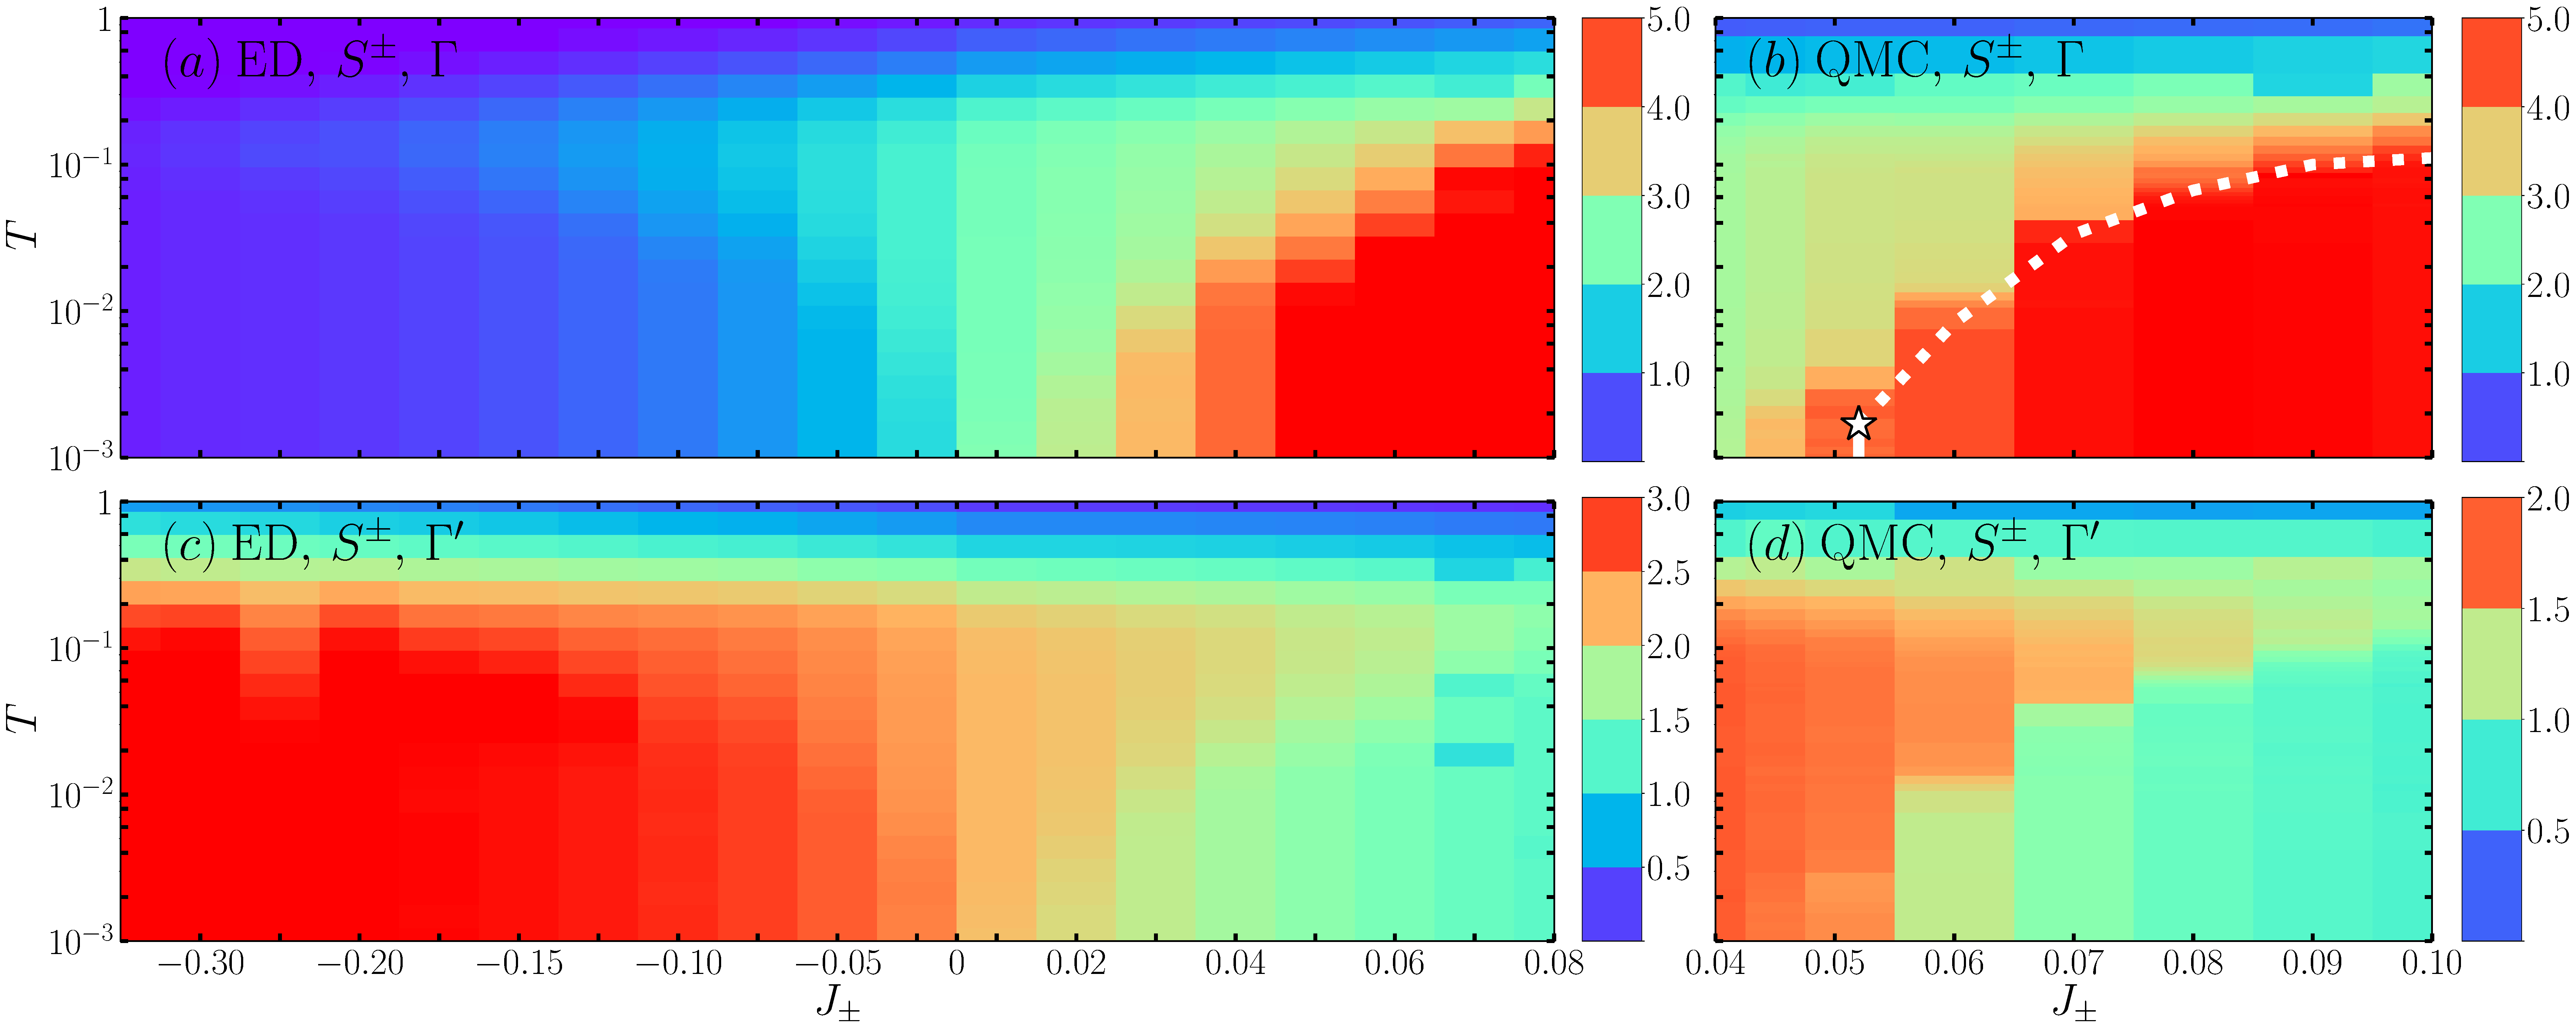
\includegraphics[width=\linewidth]{figures/Fig_2v5.pdf}
      \caption{Heat maps of the QFI as functions of temperature $T$ and $J_{\pm}$ obtained via ED (a,c) and QMC (b,d)}
      \label{fig:placeholder}
  \end{figure}
  \end{block}

  \begin{block}{Dipolar-Octupolar Compound}
  For DO compounds, the QFI associated with the experimentally accessible spectrum is the trace of the QFI with respect to the spin-flip (SF) and the non spin-flip (NSF) channels.
    \begin{subequations}
\begin{align}
    S_\mathbf{q}^{\text{NSF}} &= \sum_{\mathbf{R}_\mu} \left(\hat{\mathbf{p}}\cdot\hat{\mathbf{z}}_\mu \right)\tau^z_{\mathbf{R}_\mu}e^{i\mathbf{q}\cdot\mathbf{R}_\mu} \label{eq:op_NSF}\\
    S_\mathbf{q}^{\text{SF}} &= \sum_{\mathbf{R}_\mu} \left(\hat{\mathbf{v}}\cdot\hat{\mathbf{z}}_\mu \right)\tau^z_{\mathbf{R}_\mu}e^{i\mathbf{q}\cdot\mathbf{R}_\mu} \label{eq:op_SF}.
\end{align}
\end{subequations}
  
\begin{figure}
	\centering
	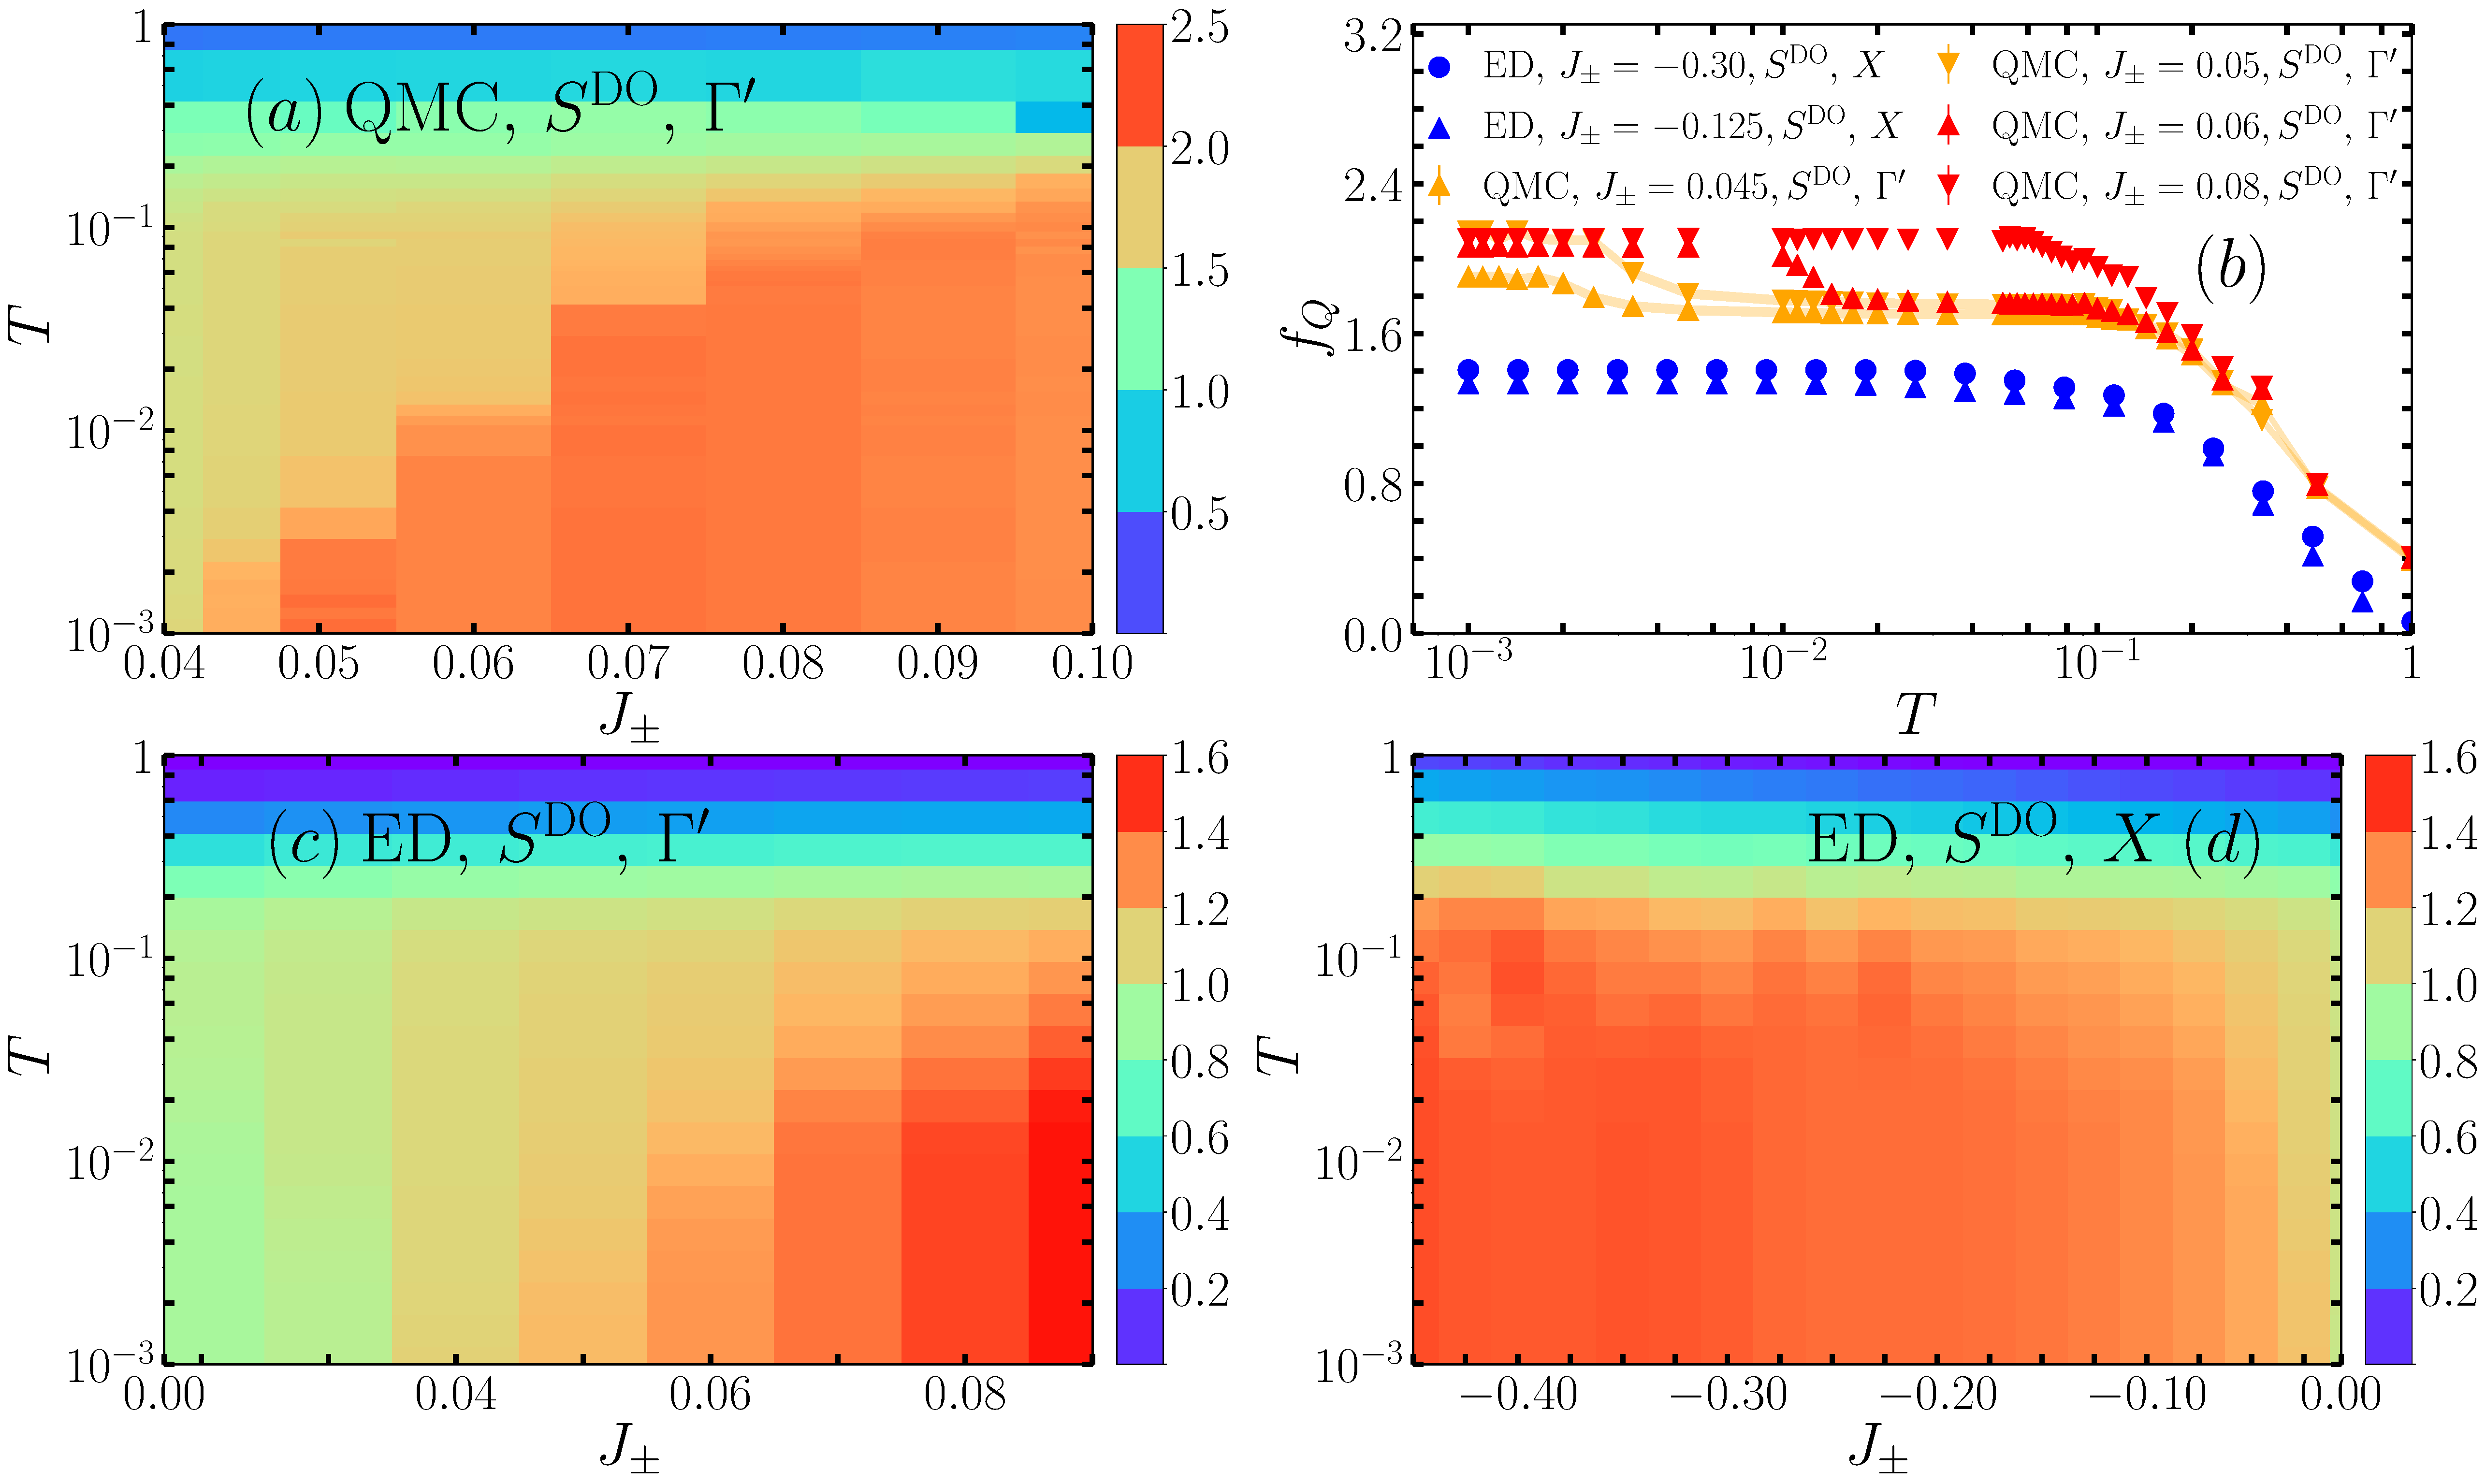
\includegraphics[width=\columnwidth]{figures/Fig_GB_3.pdf}
	\caption{\textbf{QFI in experimental coordinates for Cerium-based pyrochlore compounds.} 
    %\og{(ZCK: These results are being checked because the QMC results are not consistent with the ED data.)} 
    Panel (a) presents a heat map of the QMC computed QFI $f_{Q}(S^{\text{DO}}_{\Gamma'}, T)$, with $J_{\pm}$ ranging from $0.04$ to $0.10$. Panel (b) is the line cut of panel (a) from $J_{\pm}=0.045$ to $0.08$. The crossover temperature scales from the paramagnetic phase to CSI at $T\sim 1$ and from CSI to QSI$_0$ at $T\sim |J^3_{\pm}|$ are clearly manifest in the shaded data, highlighted in orange. Panel (c) shows ED results of $f_{Q}(S^{\text{DO}}_{\Gamma'}, T)$ for $J_{\pm}$ between $0.01$ and $0.08$. Panel (d) focuses $f_{Q}(S^{\text{DO}}_X, T)$ with $X=(0,0,2\pi)$ in the range from $-0.425$ to $0.00$.}
	\label{fig:QFI_experiment}
    \end{figure}
  \end{block}

  \begin{block}{Outlook}

    \textbf{Beyond a scalar witness.} For a pure state,
    \[
      F_Q[O] = 4\,\|\partial_{\theta}|\psi_{\theta}\rangle_{\perp}\|^2,
      \qquad |\psi_{\theta}\rangle = e^{-i\theta O}|\psi\rangle,
    \]
    so the QFI is the metric norm of the tangent vector generated by $O$.

    \begin{center}
    \resizebox{0.72\linewidth}{!}{%
    \begin{tikzpicture}[x=1cm,y=1cm,
        manifold/.style={draw=UofTLightBlue,line width=1.6mm},
        full/.style={-{Latex[length=5mm]},ultra thick,draw=UofTBlue},
        proj/.style={-{Latex[length=4mm]},line width=1.2pt},
        state/.style={circle,fill=UofTBlue,inner sep=3.2pt},
        box/.style={draw=UofTBlue,thick,rounded corners=7pt,
                    fill=UofTLightAccent,inner sep=7pt},
      ann/.style={font=\footnotesize,text=UofTBlue,align=left},
      lab/.style={font=\footnotesize\bfseries,text=UofTBlue}]
      \draw[manifold]
        plot[smooth] coordinates {(0.8,1.1) (2.0,2.35) (3.9,2.95) (5.8,2.45) (7.1,1.25)};
      \node[state] (psi) at (3.9,2.95) {};
      \node[ann,below left] at (psi) {$|\psi\rangle$};

      \draw[full] (psi) -- ++(4.35,1.35);
      \node[lab,above right] at (8.5,4.55)
        {full tangent $\partial_{\theta}|\psi_{\theta}\rangle_{\perp}$};

      \draw[proj,draw=UofTBlue!45] (psi) -- ++(1.55,0.42);
      \node[lab,below right] at (6,2.98) {$\mathcal{O}_1$};

      \draw[proj,draw=UofTBlue!65] (psi) -- ++(2.75,0.82);
      \node[lab,below right] at (6.95,3.45) {$\mathcal{O}_2$};

      \draw[proj,dashed,draw=UofTLightBlue] (psi) -- ++(4.1,1.27);
      \node[lab,below right] at (8.2,3.95) {$\mathcal{O}_{k^\star}$};

      \node[box,anchor=west] at (10.2,2.85)
        {$\mathcal{O}_1 \subset \mathcal{O}_2 \subset \cdots \subset \mathcal{O}_k$};

      \draw[-{Latex[length=4mm]},thick,UofTBlue] (13.1,2.35) -- (13.1,1.05);
      \node[ann,align=center] at (13.1,0.42)
        {increase $k$ until the restricted tangent\\recovers the full geometric direction};
    \end{tikzpicture}}
    \end{center}

    \begin{itemize}
      \item Restrict the generator to a $k$-body operator subspace $\mathcal{O}_k$.
      \item Measure how much of the tangent norm is recovered inside that subspace.
      \item The smallest $k^\star$ that saturates the tangent identifies the underlying multipartite structure.
    \end{itemize}

  \end{block}


\end{column}

\separatorcolumn
\end{columns}
\end{frame}

\end{document}
